% This is samplepaper.tex, a sample chapter demonstrating the
% LLNCS macro package for Springer Computer Science proceedings;
% Version 2.21 of 2022/01/12
%
\documentclass[runningheads]{llncs}
%
\usepackage[T1]{fontenc}
% T1 fonts will be used to generate the final print and online PDFs,
% so please use T1 fonts in your manuscript whenever possible.
% Other font encondings may result in incorrect characters.
%
\usepackage{graphicx}
\usepackage{svg}
\usepackage{booktabs}
\usepackage{float}
\usepackage{amsmath}
\usepackage{url}
\graphicspath{{figures/}}
%
% If you use the hyperref package, please uncomment the following two lines
% to display URLs in blue roman font according to Springer's eBook style:
%\usepackage{color}
%\renewcommand\UrlFont{\color{blue}\rmfamily}
%\urlstyle{rm}
%
\begin{document}
\raggedbottom
\setlength{\textfloatsep}{10pt plus 2pt minus 4pt}
\setlength{\intextsep}{8pt plus 2pt minus 4pt}
%
\title{Token-aware Agentic AI Systems: A Framework for Evaluating Token Usage Across Orchestration Approaches}
%
\titlerunning{Token-aware Agentic AI Systems}
% If the paper title is too long for the running head, you can set
% an abbreviated paper title here
%

\author{Jorge Esteban Ramirez Sashida\inst{1,2}
\orcidID{0009-0003-9003-9434} 
\and
Mauricio Diaz\inst{1,2}
\orcidID{0009-0008-4121-9697} 
\and
J. Octavio Gutierrez-Garcia\inst{1}
\orcidID{0000-0002-6252-6169}
}
%
\authorrunning{J. E. Ramirez Sashida et al.}
%
\institute{Department of Computer Science, ITAM, 01080 Mexico City, Mexico\\
\email{octavio.gutierrez@itam.mx}
\and
dive.ai, Data Science and AI Consulting Firm, 06470 Mexico City, Mexico\\
\email{\{esteban, mauricio\}@dive.ai}}
%


\maketitle              
%
% 150-250 workds
\begin{abstract}

Agentic AI systems increasingly automate enterprise workflows by leveraging large language models (LLMs) to orchestrate external tools through standardized interfaces such as the Model Context Protocol (MCP). In this domain, there are two orchestration modalities: direct invocation, where an agent calls tools sequentially and routes each intermediate result through the LLM context, and code‑execution invocation, where the agent generates a program that batches multiple tool calls within an isolated sandbox. Although direct invocation is widely adopted and code-execution invocation is an emerging approach, their efficiency trade‑offs remain insufficiently studied. This work introduces an evaluation framework for agentic AI systems that compares these orchestration modalities in both single‑agent and multi‑agent settings, using a heterogeneous task suite (including single‑tool, pipeline, and discovery tasks) across multiple MCP servers providing more than 70 tools. The framework includes an LLM‑as‑a‑judge grader and measures token consumption, task quality, and normalized efficiency. With a 0.05 significance level, empirical results indicate that code-execution invocation reduces token consumption while preserving output quality and achieving higher efficiency on complex tasks, particularly pipeline tasks, compared with direct invocation.

\keywords{Agentic AI systems \and Evaluation framework \and MCP via code execution \and Multi-agent systems.}
\end{abstract}

\section{Introduction}

Nowadays, artificial intelligence (AI) supports and automates enterprise workflows through agentic AI systems~\cite{godavarthi2026investment}, which consist of multiple agents that collaborate to carry out interconnected tasks and achieve predefined goals~\cite{sapkota2025ai}. Agents (endowed with decision-making abilities) establish a context and act toward these goals~\cite{bandi2025rise}. In recent years, to enhance their decision-making, agents leverage the reasoning capabilities of large language models (LLMs)~\cite{naveed2025comprehensive}. An LLM is a deep learning model trained on a great amount of text to perform natural language tasks~\cite{huang2024auditwen}. Unlike reactive agents, an LLM-supported agent perceives and establishes context through textual inputs and executes actions accordingly. Frequently, LLM-supported agents generate and monitor plans by interleaving reasoning traces and actions, following the ReAct framework (see~\cite{yao2022react} for details). Currently, agentic frameworks such as Amazon Bedrock, AutoGen, LangChain, and Strands Agents allow agents to invoke and orchestrate a myriad of tools and services (ranging from storage systems to AI models and web-scraping utilities) using an open model context protocol (MCP), which has been adopted as an industry standard~\cite{hou2025model}. MCP enables agents to discover and use tools in a structured manner, decoupling implementation technologies from their invocation.

With MCP providing this layer of interoperability, there are several ways to orchestrate and implement agentic systems (see~\cite{aws2025_mcp_agentcore_bedrock}). In terms of tool invocation, this article focuses on two orchestration modalities: (i) \textit{direct invocation}, in which an agent calls MCP tools one at a time, with each tool’s output added back into its context before the next call; and (ii) \textit{code-execution} invocation, in which the agent instead generates a program that invokes multiple tools inside a sandbox, processes intermediate results internally, and returns only the final output to its context.

LLM-supported agents have become increasingly effective at executing enterprise workflows under either orchestration modality. However, their performance depends in part on the amount of information (i.e., the size of the context window, measured in tokens) that an LLM can process in a single request. This constraint has motivated substantial research efforts within the scientific community (see~\cite{an2024make}, \cite{wu2024extending}, \cite{ratner2023parallel}). In this regard, in agentic AI systems executing enterprise workflows, this limitation is further amplified because, in addition to the user’s prompt, the context required for direct MCP calls must include detailed tool specifications (e.g., names, descriptions, parameters, and schemas). In practice, these tool descriptions may consume thousands of tokens (occupying a significant portion of the available context window) before an agent can even fulfill a single user request~\cite{anthropic_mcp_code_execution_2025}. Moreover, in the context of direct MCP calls, when an LLM-supported agent executes enterprise workflows involving multiple tools, all intermediate results must be routed through the context, i.e., the output of each tool becomes the input of the next, which can lead to context growth that may even exceed the available window size. 

To mitigate the above problem, the main objective of this work is twofold: first, to design an evaluation framework for agentic AI systems that compares code‑execution invocation and direct invocation as orchestration modalities; and second, to examine whether code‑execution invocation offers measurable advantages (both in token consumption and output quality) over direct invocation in agentic systems. To evaluate this, each orchestration modality was tested under both a single-agent and a multi-agent system architecture. Furthermore, to assess the implemented agentic AI systems, the agents were presented with three task types: (i) \textit{single-tool tasks}, involving a single MCP server; (ii) \textit{pipeline tasks}, involving multiple predefined MCP servers; and (iii) \textit{discovery tasks}, also involving multiple MCP servers but requiring the agent to determine which servers (and tools) to invoke. To conduct the experiments, multiple enterprise workflows (involving eight MCP servers and more than 70 tools) were created. The application domains of these servers and workflow tasks were highly heterogeneous, ranging from Morse code translation to developer utilities.

The contributions of this work are as follows.

\begin{itemize}

\item An evaluation framework for agentic AI systems across different orchestration modalities in both single-agent and multi-agent settings.

\item Empirical evidence of the trade‑offs between two widely used orchestration modalities in agentic systems, namely direct invocation and code‑execution invocation.

\item Identification of preferable orchestration modalities for different task categories, considering both token consumption and output quality.

\item A reproducible evaluation methodology for comparing orchestration modalities in agentic AI systems.
\end{itemize}

The structure of this article is as follows. Section \ref{sec:background} introduces background concepts and related work; Section \ref{sec:evaluation_framework} describes the evaluation framework; Section \ref{sec:evaluation} presents experimental settings and the empirical results; and Section \ref{sec:conclusions} provides concluding remarks.



\section{Background and Related Work}
\label{sec:background}

The rise of LLMs has accelerated research on agentic AI systems (see~\cite{raheem2025agentic}, \cite{dwivedi2026agentic}, and \cite{acharya2025agentic}), which automatically orchestrate web services (commonly referred to as \textit{tools} in this domain) to execute complex workflows. A key paradigm in this context is ReAct~\cite{yao2022react}, where agents alternate between reasoning and tool invocation. This integration of chain‑of‑thought with tool use has been shown to reduce hallucinations and improve performance on benchmarks such as HotpotQA and ALFWorld. In practice, ReAct-style tool use is commonly implemented through MCP~\cite{mcp_intro_2024}, an open protocol providing LLM‑supported agents with a uniform interface for discovering and invoking tools via JSON‑RPC 2.0. MCP is now supported by major frameworks from OpenAI, Google DeepMind, and Microsoft~\cite{hou2025model}.
However, before executing a workflow, an agent must load tool definitions into its context, which can consume tens of thousands of tokens~\cite{anthropic_advanced_tool_use_2025}. As the number of tools grows, so does the token cost of loading specifications and routing intermediate results. Since LLMs are effective at generating code~\cite{joel2024survey}, code‑execution invocation provides an alternative that reduces context growth by handling intermediate computations programmatically.



The rise of LLMs has given birth to a new research area on agentic AI systems (see~\cite{raheem2025agentic}, \cite{dwivedi2026agentic}, and \cite{acharya2025agentic}), which can automatically compose and orchestrate web services (commonly referred to as tools in this context) to execute complex enterprise workflows.

One of the most influential paradigms for agents that interact with external tools is ReAct~\cite{yao2022react}, in which agents iteratively alternate between reasoning traces and actions (i.e., tool invocations) to accomplish complex goals. In ReAct, an agent supported by an LLM deliberates, invokes a tool, observes the outcome, and then repeats this cycle. Empirical evidence indicates that integrating chain‑of‑thought reasoning with tool invocation reduces hallucinations and improves success rates on benchmarks such as HotpotQA~\cite{yang2018hotpotqa} and ALFWorld~\cite{shridhar2020alfworld}.

In industry settings, the iterative tool invocation proposed by the ReAct paradigm is commonly supported by MCP~\cite{mcp_intro_2024}, an open protocol that gives LLM-supported agents a uniform interface to invoke and discover tools exposed by external servers through JSON‑RPC 2.0. Major agentic frameworks developed by OpenAI, Google DeepMind, and Microsoft now provide MCP support for tool invocation~\cite{hou2025model}.

Using MCP and the ReAct paradigm, before executing an enterprise workflow, LLM-supported agents have to load into their context or, informally speaking, reason about the tool definitions provided by MCP servers, which, for instance, may consume up to 55,000 tokens for a scenario with five MCP servers offering 58 tools in total, before the agent conversation begins \cite{anthropic_advanced_tool_use_2025}. Consequently, as the number of tools available grows, so does the token cost of loading definitions and routing intermediate results through context. However, as LLMs have shown remarkable effectiveness in generating code~\cite{joel2024survey}, an LLM-supported agent can use code‑execution invocation to call tools from MCP servers and reduce the cost of routing intermediate results through context. 

In this context, several research efforts have been conducted to evaluate and benchmark agentic AI systems enabled by MCP. Dobriy et al.~\cite{dobriy2026agentic} evaluated LLM‑supported agents in the context of federated SPARQL querying. Their system architecture consisted of a single client communicating with a single MCP SPARQL server, primarily evaluating the validity of the generated SPARQL queries. In the domain of mobile computing, Kong et al.~\cite{kong2025mobileworld} proposed MobileWorld, a benchmark for mobile applications using agent-user interaction and MCP servers. With respect to the agentic AI system, their benchmark includes 40 tasks involving 64 tools provided by five MCP servers, evaluating task success rate and the average number of MCP calls. Mo et al.~\cite{mo2025livemcpbench} designed their benchmark to include 95 everyday tasks (e.g., lifestyle, shopping, and leisure activities), in which LLM-supported agents must interact with 70 MCP servers providing 527 tools. As before, their primary performance metric was task success rate, however, they also measured token consumption across several state‑of‑the‑art LLMs, with a particular focus on the costs associated with tool descriptions. Following a similar approach, Guo et al.~\cite{guo2026mcp} propose evaluating agentic AI systems using 600 real‑world everyday tasks (generated by LLMs but with human supervision). As in~\cite{mo2025livemcpbench}, the number of MCP servers and tools involved in the benchmark is also considerably large. It is worth mentioning that Guo et al. also propose evaluating token consumption (in addition to task success rate), however, token consumption is assessed from the perspective of the LLMs used without taking into account orchestration modalities. 

Whereas the research efforts presented in \cite{dobriy2026agentic}, \cite{kong2025mobileworld}, \cite{mo2025livemcpbench}, and \cite{guo2026mcp} are extremely valuable and contribute significantly to the evaluation of agentic AI systems, to the best of the authors' knowledge, no prior work has systematically benchmarked orchestration modalities (namely, direct invocation and code‑execution invocation) independently of the underlying AI model, with respect to both token consumption and task/output grade, which is the main focus of the present work.


\section{Evaluation Framework}
\label{sec:evaluation_framework}

The evaluation framework (Fig. \ref{fig:evaluation_framework}) consists of five main components: (i) an LLM‑supported agent; (ii) the orchestration modalities: direct invocation and code-execution invocation; (iii) a task suite; (iv) an LLM‑as‑a‑judge grader; and (v) two agent-based system architectures, namely the single‑agent and multi‑agent setups.

\begin{figure}
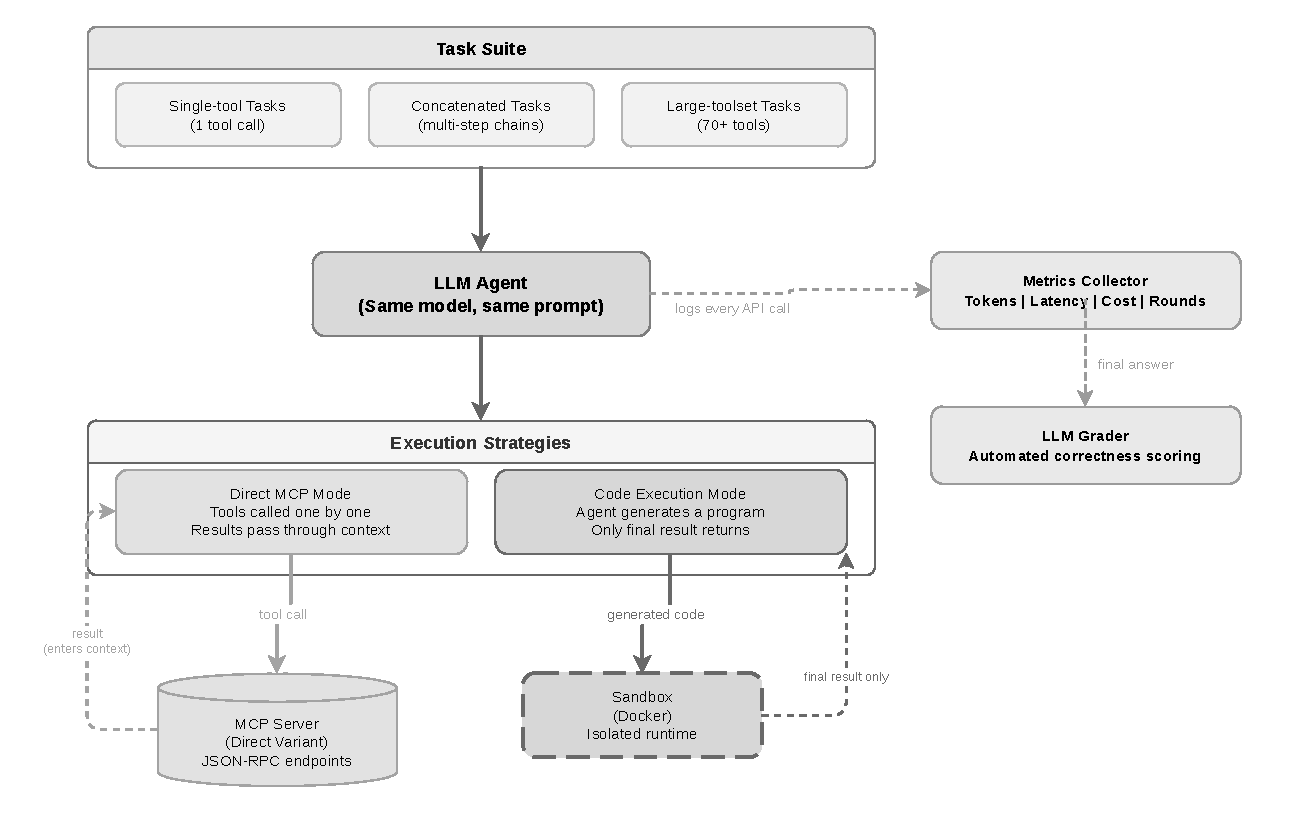
\includegraphics[width=\textwidth]{archi1.pdf}
\caption{Architectural components of the proposed evaluation framework.}
\label{fig:evaluation_framework}
\end{figure}

\subsection{LLM-supported agent}

To execute automated workflows, the LLM‑supported agent uses an AI model that receives a prompt describing a task, whose requirements must be aligned with the capabilities of the available MCP servers. The LLM‑supported agent also includes a metrics collector to track token usage, success rate, and other relevant performance metrics.

\subsection{Orchestration modalities}

The LLM-supported agent can make use of two orchestration modalities: 

\begin{itemize}

    \item \textit{Direct invocation} (DI), in which the agent invokes tools individually and sequentially using direct MCP calls, and each call's output (i.e., the emitted tokens) is appended to the agent’s context before executing the next call. Using  FastMCP, the agent calls the tools (exposed as JSON endpoints) via streamable HTTP or standard I/O calls.
    
    \item \textit{Code-execution invocation} (CI), in which the agent generates a program (treating MCP tools as code APIs that can be invoked programmatically) to orchestrate multiple tool calls within a (Docker) sandbox where the agent executes the code. This allows intermediate results to be processed programmatically within the generated code, and only the final program output, i.e., the resulting tokens, is returned to the agent’s context. In addition, inside the Docker container, Python files describe the corresponding MCP tools and a dependency list ensures the agent can import and execute these tools within the sandbox.

\end{itemize}

\subsection{Task suite}
\label{sec:task_suite}


The task suite executed by the LLM‑supported agent comprises 54 tasks across three task types, each designed to reflect increasing levels of operational complexity:


\begin{itemize}

  \item \textit{Single-tool}. Tasks where an MCP server exposes a single tool for a straightforward input-output operation. These tasks provide a baseline for comparing the overhead of code‑execution invocation against the minimal overhead of a direct MCP call. Examples of single-tool tasks include translating a string to Morse code and searching for an artist on LastFM.
    
  \item \textit{Pipeline}. Tasks where an MCP server exposes multiple tools and the agent must chain their outputs sequentially to complete the task. In these tasks, the agent must determine the correct sequence of tool calls and combine them appropriately. An example of a pipeline task is listing an artist's albums on LastFM and then getting the most popular track for each album.
  
  \item \textit{Discovery}. Tasks involving 50 or more tools within a single MCP server, requiring the agent to explore the available tools and select the appropriate ones. These tasks may involve either single‑tool or pipeline tasks. An example of a discovery task is converting a string using the correct utility from an MCP server containing 60 or more tools.
    
\end{itemize}

Nine MCP servers are available to execute the tasks. Each server corresponds to a specific application domain and exposes a different number of tools. Table~\ref{tab:servers} summarizes the servers used in the evaluation framework.

\begin{table}
\caption{MCP server domains and tool counts.}\label{tab:servers}
\centering
\begin{tabular}{|l|l|p{6cm}|}
\hline
\textbf{MCP Server} & \textbf{Number of tools} & \textbf{Description} \\
\hline
Morse & 1 & Simple morse code translation \\
Cocktails & 3 & Cocktail recipe search \\
Postgres & 3 & Database operations \\
NASA & 4 & NASA image/video search and metadata \\
AlphaVantage & 4 & Stock market data  \\
Nutrition & 5 & Nutritional information lookup \\
LastFM & 26 & Music discovery \\
DevToolkit & 60+ & Developer utilities \\
Cross-Server & Varies & Tasks requiring multiple servers \\
\hline
\end{tabular}
\end{table}

The servers were selected to represent different levels of workflow complexity. The Morse MCP server is the simplest case, exposing a single tool with a straightforward input-output mapping. The DevToolkit MCP server represents the large‑toolset scenario, offering more than 60 tools. Postgres and Cross‑Server, in contrast, support tasks requiring multi-step reasoning and coordination across multiple MCP tools or servers.

In addition, to evaluate whether the number of connected MCP servers affects performance, each task was executed under three server-load conditions: (i) \textit{minimal}, where only the server(s) required for the task are connected; (ii) \textit{moderate}, where the required server(s) plus a few distractor servers with unrelated tools are connected; and (iii) \textit{maximal}, where the required server(s) plus all remaining servers act as distractors. This setup allows assessing whether loading additional tool definitions into the context degrades performance (one of the key motivations for \textit{code-execution} invocation).

\subsection{LLM-as-a-judge grader}

The grader receives a rubric specifying how each task should be evaluated and assesses whether the LLM‑supported agent produced the correct result with the appropriate level of detail. The rubric includes the task objective and the expected output. Once the LLM-supported agent completes a task, its output is submitted to the LLM-as-a-judge grader, which assigns a score from 0 (lowest) to 1 (highest).

\subsection{Agent-based system architectures}

The evaluation framework supports two agent-based system architectures: single-agent architecture and multi-agent architecture. Both system architectures can be implemented in Amazon Bedrock~\cite{aws_bedrock_2026}.

\begin{itemize}

    \item The \textit{single-agent} architecture is implemented using a \textit{Strands} agent supported by an LLM. The agent receives a prompt that connects the AI model to the available MCP tools required for completing the task. In this setup, the agent has access to all necessary MCP servers. Under \textit{direct invocation}, the Strands agent calls each tool individually via JSON-RPC, appending every result to its context. Under \textit{code‑execution invocation}, the agent generates a program that runs inside a Docker sandbox, where the MCP tools are available as importable Python modules. Only the final program output is returned to the agent’s context.

    \item The \textit{multi-agent} architecture is implemented using a \textit{Strands} agent orchestrator. The orchestrator receives the task and delegates subtasks to specialized subordinate agents, each assigned to a specific MCP server. Under \textit{direct invocation}, each subordinate agent calls its corresponding MCP server via JSON-RPC and returns its results to the orchestrator. Under \textit{code‑execution invocation}, each subordinate agent operates in its own isolated Docker sandbox containing the necessary tool files and dependencies, returning only the final output. No state is shared between sandboxes.

\end{itemize}


\section{Evaluation and Empirical Results}
\label{sec:evaluation}

\subsection{Experimental settings}

\subsubsection{Agent-based system configurations.} To determine whether \textit{code‑execution invocation} offers measurable advantages over \textit{direct invocation} in agentic AI systems, the task suite described in Section~\ref{sec:task_suite} was executed using four agent configurations (Fig.~\ref{fig:system_configurations}):

\begin{figure}
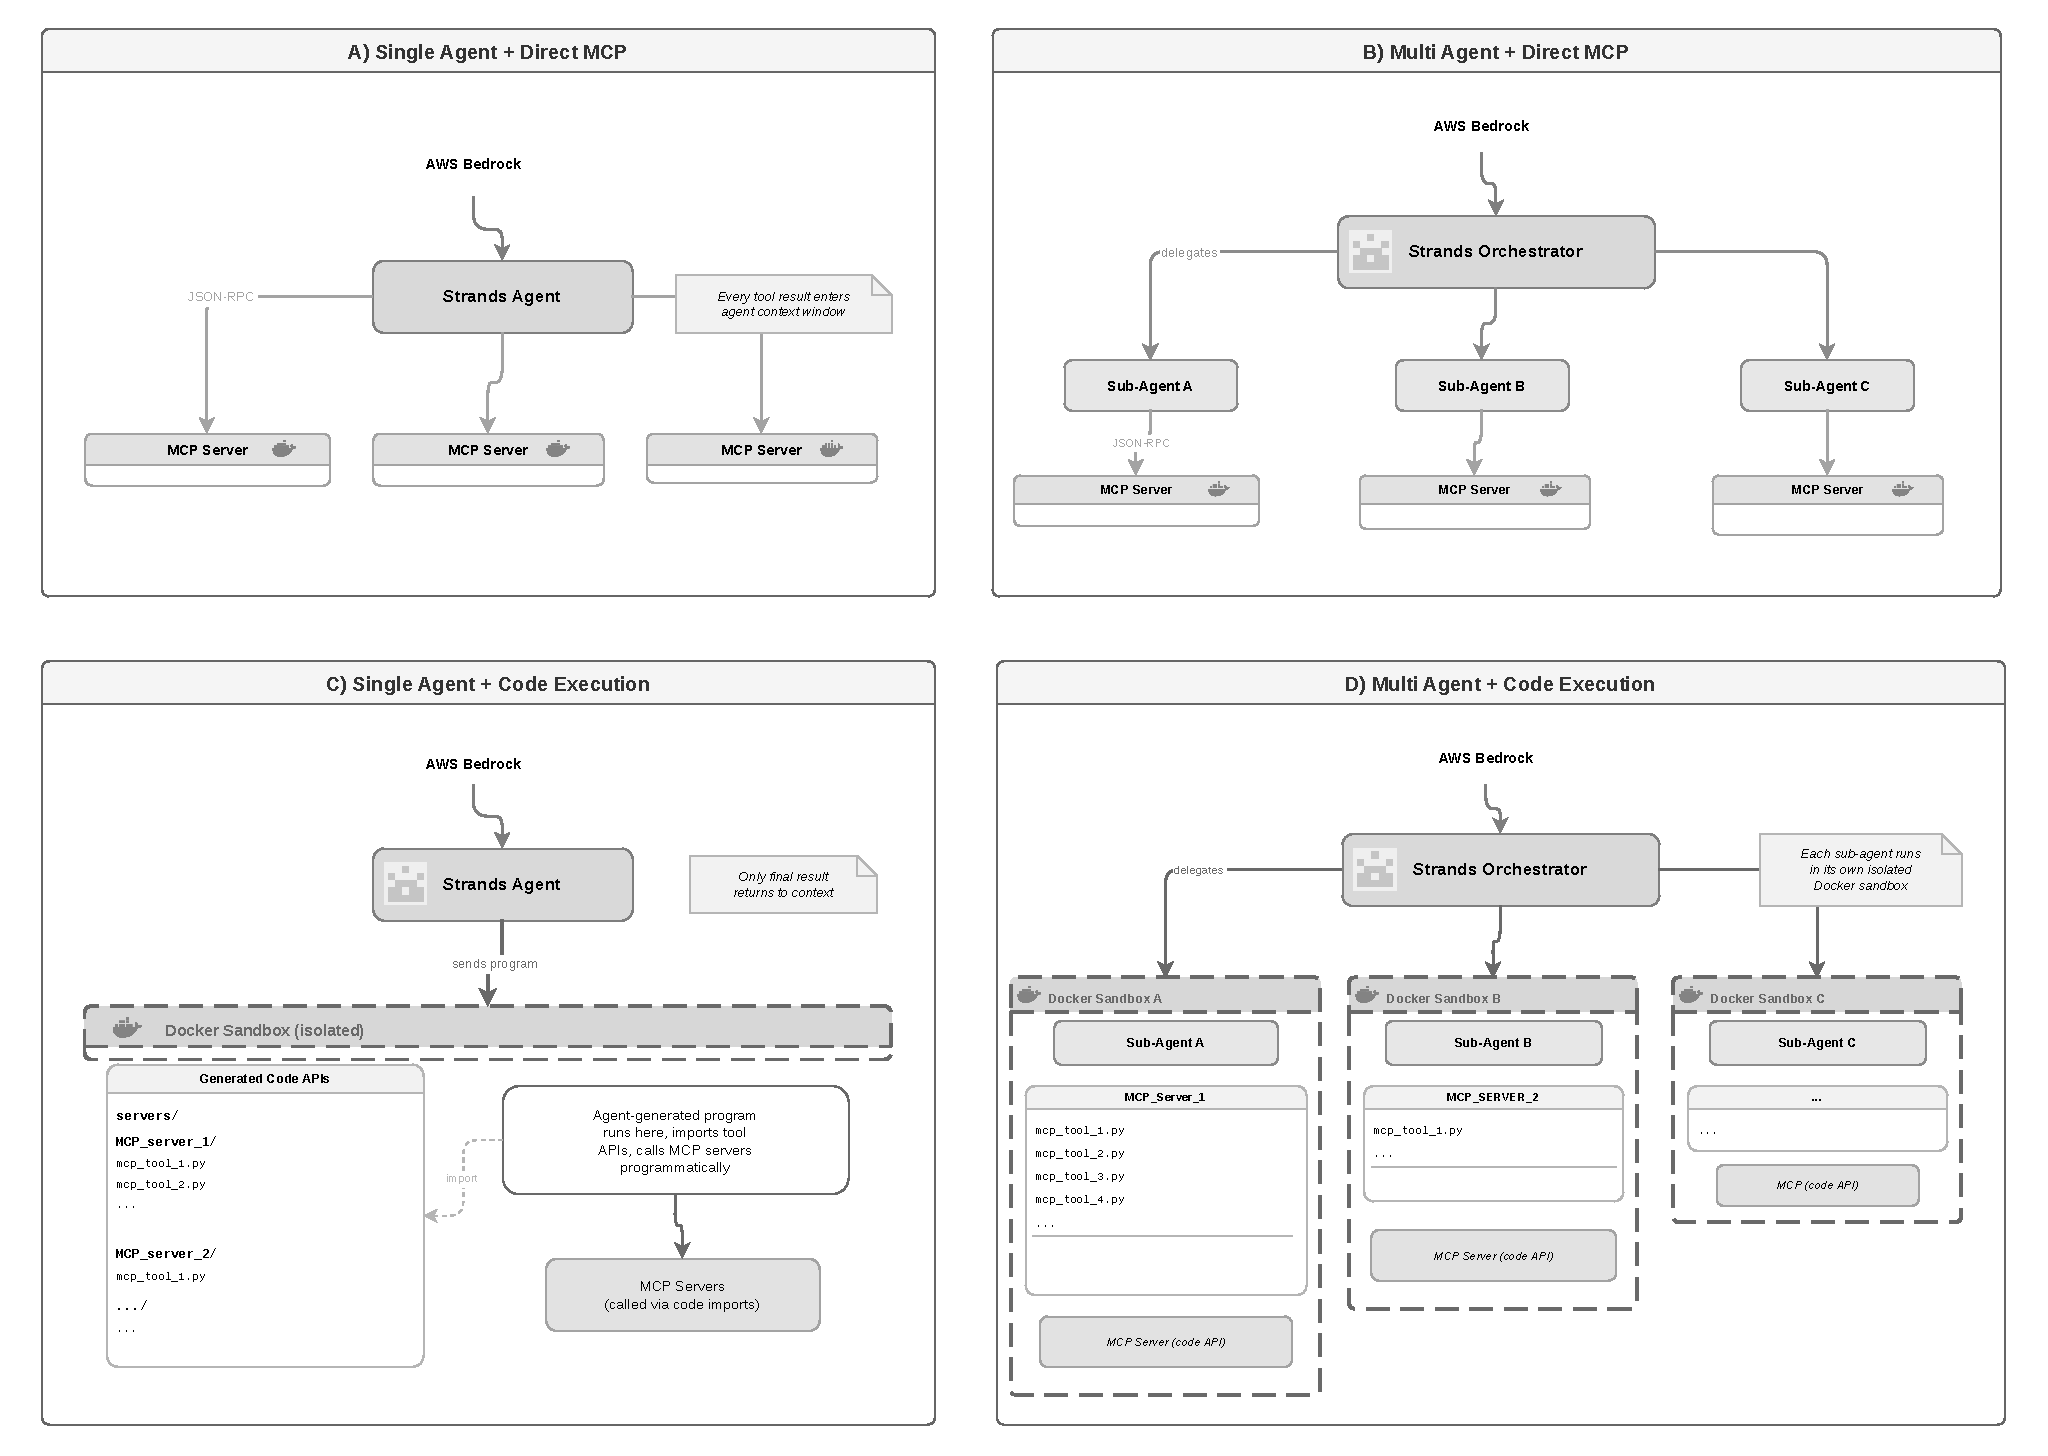
\includegraphics[width=\textwidth]{archi2.pdf}
\caption{Overview of the agentic AI system configurations.}
\label{fig:system_configurations}
\end{figure}

\begin{itemize}
    \item \textit{Single-agent DI}: Single-agent architecture using direct invocation.
    \item \textit{Single-agent CI}: Single-agent architecture using code‑execution invocation.
    \item \textit{Multi-agent DI}: Multi-agent architecture using direct invocation.
    \item \textit{Multi-agent CI}: Multi-agent architecture using code‑execution invocation.
\end{itemize}

\subsubsection{Supporting LLM.} All four configurations use Claude 3.7 Sonnet through AWS Bedrock with a temperature of 0.2 and the same system prompt.

\subsubsection{Performance measures.}
Each task execution was evaluated using three metrics:

\begin{itemize}
    \item \textit{Task grade}: A score from 0 to 1 assigned by the LLM-as-a-judge grader.
    \item \textit{Token usage}: Total input and output tokens consumed across all LLM calls for a given task.
    \item \textit{Efficiency}: Grade per 1,000 tokens, capturing the trade-off between output quality and token cost.
\end{itemize}

\subsubsection{Experiment runs.} The full experiment consisted of 582 task executions across the four system configurations (Fig.~\ref{fig:system_configurations}), eight MCP servers (Table~\ref{tab:servers}), three task types (single‑tool, pipeline, discovery), and three server-load conditions (minimal, moderate, maximal). It should be noted that results from the AlphaVantage MCP server were excluded due to persistent rate-limiting failures. 

Table~\ref{tab:config} summarizes the experimental configuration.

\begin{table}[H]
\caption{Summary of experimental settings}\label{tab:config}
\centering
\begin{tabular}{|l|l|}
\hline
\textbf{Parameter} & \textbf{Possible values} \\
\hline
AI model      & Claude 3.7 Sonnet \\
Temperature   & 0.2 \\
Total runs    & 582 \\
MCP servers   & 8 \\
Task types    & 3 (single‑tool, pipeline, discovery) \\
Agent types   & 4 (single‑agent DI/CI, multi‑agent DI/CI) \\
Load levels   & 3 (minimal, moderate, maximal) \\
\hline
\end{tabular}
\end{table}

\subsubsection{Empirical results.} From the series of experiments, three main observations were obtained. To facilitate interpretation, the results (presented in Figs.~\ref{fig:grade}-\ref{fig:tokens} and Tables~\ref{tab:efficiency} and \ref{tab:tokens}) were grouped by task type and orchestration modality. A p-value less than 0.05 was considered significant. 

% ----- 1. GRADE -----
\textit{Observation 1: Task grade.} Agents using direct invocation achieved a higher overall mean grade (0.944) compared with agents using code-execution invocation (0.922), with discovery tasks showing the largest difference (see Fig.~\ref{fig:grade}).

\begin{figure}[H]
\centering
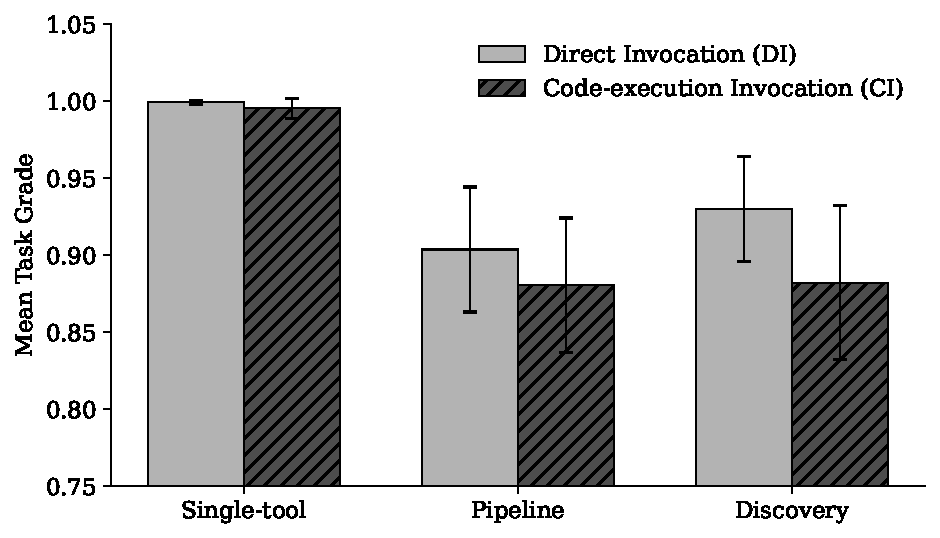
\includegraphics[width=0.7\textwidth]{eval_grade_by_mode_task.pdf}
\caption{Mean task grade by invocation modality and task type. Error bars indicate 95\% confidence intervals.}
\label{fig:grade}
\end{figure}


\textit{Analysis}. Although agents using direct invocation consistently outperformed those using code-execution invocation in raw grade, a one‑way ANOVA indicates no significant main effect of orchestration modality on task grade ($F = 2.456$, $p = 0.118$). This suggests that code-execution invocation preserves output quality while potentially offering the cost advantages examined below.

% ----- 2. EFFICIENCY -----
\textit{Observation 2: Normalized efficiency}. Agents using code-execution invocation are significantly more efficient on pipeline and discovery tasks, but less efficient on single‑tool tasks (see Fig.~\ref{fig:efficiency} and Table ~\ref{tab:efficiency}).

\begin{figure}[H]
\centering
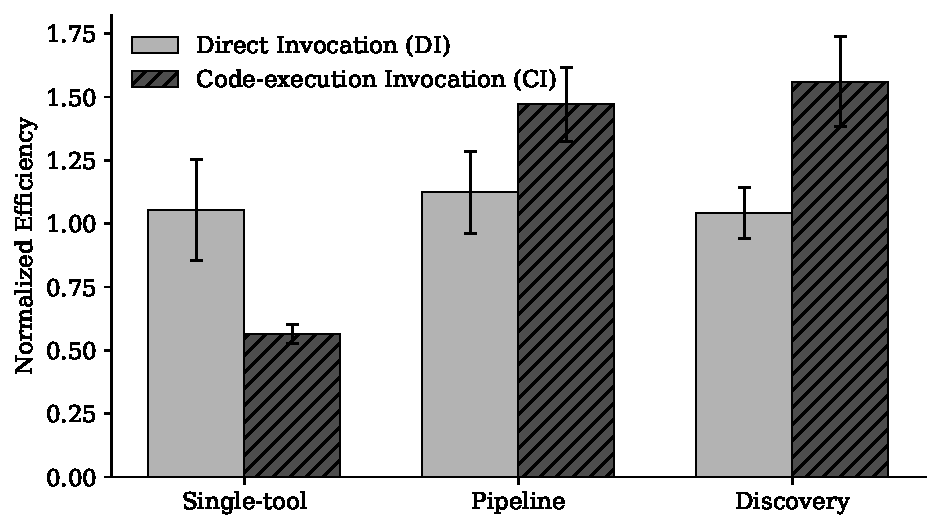
\includegraphics[width=0.7\textwidth]{eval_efficiency_by_mode_task.pdf}
\caption{Normalized efficiency by invocation modality
and task type. Error bars indicate 95\% confidence intervals. Efficiency was normalized such that single-agent DI equals 1.0 within each task type}
\label{fig:efficiency}
\end{figure}

\begin{table}[H]
\caption{Normalized efficiency by invocation modality and task type.}\label{tab:efficiency}
\centering
\begin{tabular}{|l|c|c|c|c|c|}
\hline
\textbf{Task type} & \textbf{DI} & \textbf{CI} & $t$ & $p$ & $d$ \\
\hline
Single-tool & $1.055 \pm 0.198$ & $0.564 \pm 0.037$ & $-4.823$ & ${<}0.001$ & $-0.675$ \\
Pipeline    & $1.123 \pm 0.163$ & $1.472 \pm 0.146$ &  3.162 & 0.002  &  0.430 \\
Discovery   & $1.042 \pm 0.100$ & $1.560 \pm 0.178$ &  5.059 & ${<}0.001$ &  0.803 \\
\hline
\end{tabular}
\end{table}
\textit{Analysis}. Agents using code-execution invocation were more efficient on both pipeline and discovery tasks due to their ability to batch multiple operations within a single program, thereby reducing the cumulative token-usage overhead associated with sequential direct MCP calls. This yields up to a 1.5× improvement in quality‑per‑token. The effect is particularly pronounced for discovery tasks ($d = 0.803$, large), as the programmatic enumeration of tools in code‑execution invocation avoids repeatedly loading all tool schemas into the agent’s context.

\textit{Observation 3 - Token usage.} Agents using direct invocation consumed an average of 31,161 tokens, compared with 21,576 tokens for agents using code‑execution invocation (a $1.44\times$ reduction). These savings are statistically significant for pipeline tasks, but not for single‑tool or discovery tasks (see Fig.~\ref{fig:tokens} and Table ~\ref{tab:tokens}).

\begin{figure}[H]
\centering
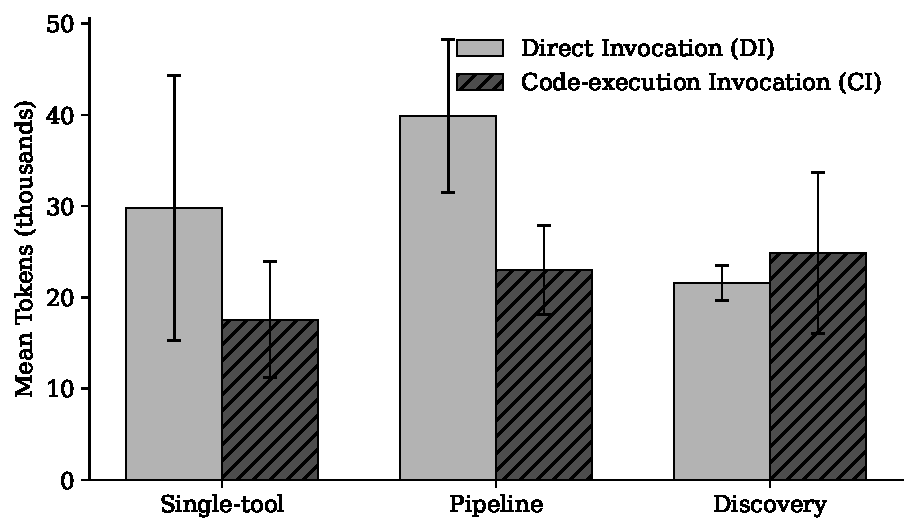
\includegraphics[width=0.7\textwidth]{eval_tokens_by_mode_task.pdf}
\caption{Mean token usage (in thousands) by invocation modality and task type. Error bars indicate 95\% confidence intervals.}
\label{fig:tokens}
\end{figure}

\begin{table}[H]
\caption{Mean token usage (in thousands) by invocation modality and task type.}\label{tab:tokens}
\centering
\begin{tabular}{|l|c|c|c|c|c|}
\hline
\textbf{Task type} & \textbf{DI} & \textbf{CI} & $t$ & $p$ & $d$ \\
\hline
Single-tool & $29.8 \pm 14.5$ & $17.5 \pm 6.4$  & 1.538 & 0.126  & 0.215 \\
Pipeline    & $39.9 \pm 8.3$  & $23.0 \pm 4.9$  & 3.453 & ${<}0.001$ & 0.470 \\
Discovery   & $21.6 \pm 1.9$  & $24.9 \pm 8.8$  & $-0.728$ & 0.469  & $-0.116$ \\
\hline
\end{tabular}
\end{table}

\textit{Analysis}. Agents using code-execution invocation achieved the largest token savings on pipeline tasks (Fig.~\ref{fig:tokens}), supporting the theoretical argument presented in~\cite{anthropic_mcp_code_execution_2025}: batching sequential tool calls within a single code-execution step avoids the token overhead of routing each intermediate result through the LLM context. However, for discovery tasks, agents using code-execution invocation consumed a similar number of tokens as those using direct invocation, likely due to the additional overhead of a single agent managing a large toolset. A one‑way ANOVA ($F = 7.205$, $p = 0.008$) confirms that invocation modality has a significant effect on token consumption when considered in aggregate.

\section{Conclusions}
\label{sec:conclusions}

This work provides the first empirical comparison of two widely used orchestration modalities in agentic AI systems: direct invocation and code-execution invocation. In addition, it introduces an evaluation framework for assessing orchestration strategies in terms of token usage and task quality, using a heterogeneous task suite and an LLM-as-a-judge grader across both single‑ and multi‑agent architectures.

The empirical results show that code-execution invocation reduces token consumption while preserving output quality. Moreover, it achieves higher efficiency on complex tasks, particularly pipeline tasks, when compared with direct invocation.

As a direction for future work, experiments with different state‑of‑the‑art AI models are planned to explore potential model‑dependent performance differences.


\begin{credits}

\subsubsection{\ackname}

The authors gratefully acknowledges the financial support from the Asociacion Mexicana de Cultura, A.C. and the technical support from Sofía Maldonado, Pablo Roca, and Miguel Quintero. It is acknowledged that grammar was checked and adjusted using Microsoft Copilot.


\subsubsection{\discintname}
The authors have no competing interests to declare that are relevant to the content of this article.
\end{credits}



\bibliographystyle{splncs04}
\bibliography{mybibliography}


\end{document}
